\documentclass{article}

\usepackage{fancyhdr}
\usepackage{extramarks}
\usepackage{amsmath}
\usepackage{amsthm}
\usepackage{amsfonts}
\usepackage{tikz}
\usepackage[plain]{algorithm}
\usepackage{algpseudocode}
\usepackage{filecontents}
\usepackage{pgfplots}
\usepgfplotslibrary{statistics}
\usepackage{mathtools}

% \usepackage{polski}
% \usepackage[utf8]{inputenc}

\usetikzlibrary{automata,positioning}

%
% Basic Document Settings
%

\topmargin=-0.45in
\evensidemargin=0in
\oddsidemargin=0in
\textwidth=6.5in
\textheight=9.0in
\headsep=0.25in

\linespread{1.1}

\pagestyle{fancy}
\lhead{\hmwkAuthorName}
\chead{\hmwkClass\ (\hmwkClassInstructor\ \hmwkClassTime): \hmwkTitle}
\rhead{\firstxmark}
\lfoot{\lastxmark}
\cfoot{\thepage}

\renewcommand\headrulewidth{0.4pt}
\renewcommand\footrulewidth{0.4pt}

\setlength\parindent{0pt}

%
% Create Problem Sections
%

\newcommand{\enterProblemHeader}[1]{
    \nobreak\extramarks{}{Problem \arabic{#1} continued on next page\ldots}\nobreak{}
    \nobreak\extramarks{Problem \arabic{#1} (continued)}{Problem \arabic{#1} continued on next page\ldots}\nobreak{}
}

\newcommand{\exitProblemHeader}[1]{
    \nobreak\extramarks{Problem \arabic{#1} (continued)}{Problem \arabic{#1} continued on next page\ldots}\nobreak{}
    \stepcounter{#1}
    \nobreak\extramarks{Problem \arabic{#1}}{}\nobreak{}
}

\setcounter{secnumdepth}{0}
\newcounter{partCounter}
\newcounter{homeworkProblemCounter}
\setcounter{homeworkProblemCounter}{1}
\nobreak\extramarks{Problem \arabic{homeworkProblemCounter}}{}\nobreak{}

%
% Homework Problem Environment
%
% This environment takes an optional argument. When given, it will adjust the
% problem counter. This is useful for when the problems given for your
% assignment aren't sequential. See the last 3 problems of this template for an
% example.
%
\newenvironment{homeworkProblem}[1][-1]{
    \ifnum#1>0
        \setcounter{homeworkProblemCounter}{#1}
    \fi
    \section{Problem \arabic{homeworkProblemCounter}}
    \setcounter{partCounter}{1}
    \enterProblemHeader{homeworkProblemCounter}
}{
    \exitProblemHeader{homeworkProblemCounter}
}

%
% Homework Details
%   - Title
%   - Due date
%   - Class
%   - Section/Time
%   - Instructor
%   - Author
%

\newcommand{\hmwkTitle}{Assignment\ \#1}
\newcommand{\hmwkDueDate}{Novermber 2017}
\newcommand{\hmwkClass}{Information Theory}
\newcommand{\hmwkClassInstructor}{Marek Smieja}
\newcommand{\hmwkAuthorName}{\textbf{Szymon Maszke}}

%
% Title Page
%

\title{
    \vspace{2in}
    \textmd{\textbf{\hmwkClass:\ \hmwkTitle}}\\
    \normalsize\vspace{0.1in}\small{Due\ on\ \hmwkDueDate\ at 3:10pm}\\
    \vspace{0.1in}\large{\textit{\hmwkClassInstructor\ \hmwkClassTime}}
    \vspace{3in}
}

\author{\hmwkAuthorName}
\date{}

\renewcommand{\part}[1]{\textbf{\large Part \Alph{partCounter}}\stepcounter{partCounter}\\}

%
% Various Helper Commands
%

% Useful for algorithms
\newcommand{\alg}[1]{\textsc{\bfseries \footnotesize #1}}

% For derivatives
\newcommand{\deriv}[1]{\frac{\mathrm{d}}{\mathrm{d}x} (#1)}

% For partial derivatives
\newcommand{\pderiv}[2]{\frac{\partial}{\partial #1} (#2)}

% Integral dx
\newcommand{\dx}{\mathrm{d}x}

% Alias for the Solution section header
\newcommand{\solution}{\textbf{\large Solution}}

% Probability commands: Expectation, Variance, Covariance, Bias
\newcommand{\E}{\mathrm{E}}
\newcommand{\Var}{\mathrm{Var}}
\newcommand{\Cov}{\mathrm{Cov}}
\newcommand{\Bias}{\mathrm{Bias}}

\begin{document}

\maketitle

\pagebreak

\begin{homeworkProblem}
  Given roll consisting of two dices and two events:
  \begin{enumerate}
    \item \(A\) even sum of roll
    \item \(B\) even product of roll
  \end{enumerate}
   calculate \(P(A|B)\). Are those events independent?\\


  \solution\\

    \part\\
    We calculate probabilities for even sum of roll and even product of roll.
      \begin{table}[h]
      \centering
      \caption{Sum of rolls}
      \begin{tabular}{|c|ccccccc}
      & 1 & 2 & 3 & 4  & 5  & 6 \\
      \hline
      1 & 2 & 3 & 4 & 5  & 6  & 7  \\
      2 & 3 & 4 & 5 & 6  & 7  & 8  \\
      3 & 4 & 5 & 6 & 7  & 8  & 9  \\
      4 & 5 & 6 & 7 & 8  & 9  & 10 \\
      5 & 6 & 7 & 8 & 9  & 10 & 11 \\
      6 & 7 & 8 & 9 & 10 & 11 & 12
      \end{tabular}
      \end{table}

    For two undistinguishable dices probablity of their sum being even is equal
    to $P(A) = \frac{12}{36} $.

      \begin{table}[h]
      \centering
      \caption{Product of rolls}
      \begin{tabular}{|c|ccccccc}
      & 1 & 2 & 3 & 4  & 5  & 6 \\
      \hline
      1 & 1 & 2 & 3 & 4  & 5  & 6  \\
      2 & 2 & 4 & 6 & 8  & 10 & 12  \\
      3 & 3 & 6 & 9 & 12  & 15  & 18  \\
      4 & 4 & 8 & 12 & 16  & 20  & 24 \\
      5 & 5 & 10 & 15 & 20  & 25 & 30 \\
      6 & 6 & 12 & 18 & 24 & 30 & 36
      \end{tabular}
      \end{table}

    For two undistinguishable dices probablity of their product being even is equal
    to $P(B) = \frac{15}{36} $.
    \\

    \part\\
    We calculate \(P(A|B)\).\\\\
    Given $P(A|B) = \frac{P(A,B)}{P{B}}$ and $P(A,B) = \frac{4}{36}$\\
    the conditional probability is: $P(A|B) =
    \frac{\frac{4}{36}}{\frac{15}{36}}$ which equals
    $P(A|B) = \frac{4}{15}$\\

    \part\\
    We test events independence based on condition: $A \perp B = P(A)*P(B)$\\
    Given $P(A) = \frac{12}{36}$ and $P(B) = \frac{15}{36}$ we conclude that
    $P(A)*P(B) = \frac{15}{108}$.\\\\
    Based on those results $\frac{15}{108} \neq \frac{4}{36}$ thus A and B are not
    independent events

\end{homeworkProblem}

\pagebreak

\begin{homeworkProblem}
    Distribution of vector $(X,Y)$ is given by the following table:
      \begin{table}[h]
      \centering
      \begin{tabular}{|c|ccccc}
      $X,Y$ & 1 & 2 & 3 & 4 \\
      \hline
      1 & 0.1 & 0.2 & 0.1 & 0 \\
      2 & 0.3 & 0 & 0.2 & 0.1 \\
      \end{tabular}
      \end{table}
    \\
    Are $X,Y$ independent? Find marginal distributions. Calculate distribution
    $X|Y = 1$ and it's mean. \\

    \solution\\
    \\
    \part\\
    We calculate marginal distributions based on equation:
    \begin{equation}
      P(X) = \sum_{y}P(X,Y) = \sum_{y}P(X|Y=y)P(Y=y)
    \end{equation}
    Marginal distribution for X is therefore given by:
    \begin{align}
      P(X=1) &= P(X=1|Y=1) + \cdots + P(X=1|Y=4) =
      0.1 + 0.2 + 0.1 = 0.4\\
      P(X=2) &= \cdots = 0.3 + 0.2 + 0.1 = 0.6
    \end{align}
    Therefore marginal distribution of X is given by vector $[0.4, 0.6]$\\
    Analougous calculations for Y give us marginal distribution described by
    vector: $[0.4, 0.2, 0.3, 0.1]$\\

    \part\\
    We test events independence based on condition: $X \perp Y = P(X)*P(Y)$\\\\
    Given $P(X=1, Y=1)=0.1$ let's calculate $P(X=1)*P(Y=1)$ which equals to
    $0.4*0.4 = 0.16$\\\\
    We can see that $P(X=1, Y=1) \neq P(X=1)*P(Y=1)$ therefore those events are
    not linearly independent based on the condtion.\\\\
    \part\\
    Distribution of X given Y = 1 is given by vector $[0.1, 0.3]$ and it's mean
    is $\frac{0.1 + 0.3}{2} = 0.2$

\end{homeworkProblem}

\pagebreak

\begin{homeworkProblem}
  Defectiveness of certain product is 10\%. You sample 3 pieces of
  forementioned. Derive distribution of random variable describing the number of
  defective products sampled.\\

  \solution\\

  \textbf{In the following section defective sample will be indicated by $D$ and
  non-defective by $O$}\\\\
  We have four possible outcomes of forementioned sampling:
  \begin{itemize}
    \item None of the products are defective
    \item One of the products is defective
    \item Two of the products are defective
    \item Every product is defective
  \end{itemize}

  For each of those events we have to calculate probability of event's
  occurence, therefore:
  \begin{itemize}
    \item $P(O, O, O) = 0.9 * 0.9 * 0.9 = 0.729$
    \item Probability of one defective product is given by:\\
      $P(D,O,O) + P(O,D,O) + P(O,O,D) = 0.1*0.9*0.9 * 3 = 0.243$
    \item Probability of two defective products is given by:\\
      $P(O,D,D) + P(D,O,D) + P(D,D,O) = 0.9*0.1*0.1*3 = 0.027$
    \item $P(D,D,D) = 0.1 * 0.1 * 0.1 = 0.001$
  \end{itemize}

  Summing the above:
  \begin{align}
    P(O,O,O) + P(D,O,O)*3 + P(O,D,D)*3 + P(D,D,D) = 1
  \end{align}
  proves correctness of the assumption about possible outcomes for this
  event.\\

\textbf{Therefore distribution of product's defectiveness with 3 samples is given by
vector}:\\\\
\centerline{$[0.729, 0.243, 0.027, 0.001]$}

\begin{figure}[!h]
\centering
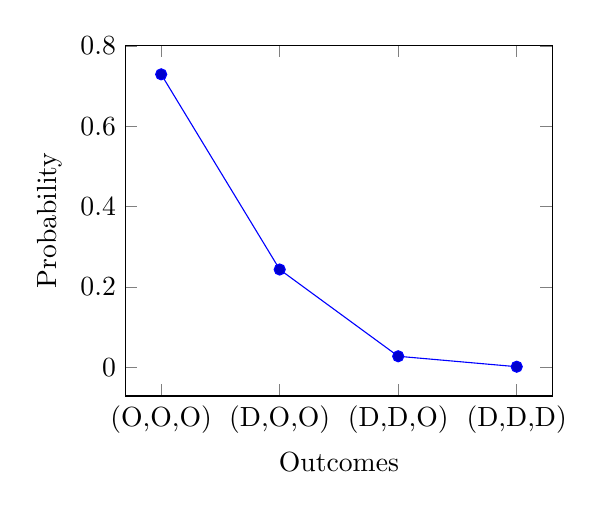
\begin{tikzpicture}
    \begin{axis}
        [
        ,width=7cm
        ,xlabel=Outcomes
        ,ylabel=Probability
        ,xtick=data,
       %,xtick={0,1,...,3}
        ,xticklabels={(O,O,O),(D,O,O),(D,D,O),(D,D,D)}
        ]
        \addplot+[sharp plot] coordinates
        {(0,0.729) (1,0.243) (2,0.027) (3,0.001)};
    \end{axis}
\end{tikzpicture}
\end{figure}

\end{homeworkProblem}

\pagebreak

\begin{homeworkProblem}
  Two certain machines are available on the market; 60\% produced by
  company A and 40\% by company B. 2\% of A's machines are defective and 1\% of
  B's.\\
  Calculate:
  \begin{itemize}
    \item Sampled machine is created by company A and is defective
    \item Probability of machine's defectiveness
    \item If machine is defective, what is the probability of it coming from A
  \end{itemize}

  \solution\\\\
  Solutions to each problem provided in the same order:
      \begin{itemize}
        \item $P(A, D) = 0.6*0.02 = 0.012$
        \item We have to sum probabilities of defectiveness from different companies:\\
          $P(D) = P(A,D) + P(B,D) = 0.012 + 0.4*0.01 = 0.016$
        \item We have to use conditional probability and Bayes Rule, for this
          example taking the form of:\\
          $P(A|D) = \frac{P(A)*P(D|A)}{P(A)*P(D|A) + P(B)*P(D|B)}$, so:\\
          $P(A|D) = \frac{0.6*0.2}{0.6*0.2 + 0.4*0.1} = 0.75$

      \end{itemize}

\end{homeworkProblem}

\pagebreak

\begin{homeworkProblem}[8]
  We have 100 workes whose seniority follows normal distribution $\mathcal{N}(10,
  5)$.\\ Calculate workers whose seniority is:
  \begin{itemize}
    \item Shorter than 3 years $P(X<3)$
    \item Between 3 and 5 years $P(3<X<5)$
  \end{itemize}
  \solution\\\\
  First we have to standardize our distribution to obtain easily intepretable z
  values.
  For standarization we need the mean of distribution and standard deviation and
  follow the formula:
  \begin{align}
    z = \frac{x - \mu}{\sigma}
  \end{align}
  \begin{itemize}
    \item for 3: $z = \frac{3 - 10}{5} = -1.4$
    \item for 5: $z = \frac{5 - 10}{5} = -1$
  \end{itemize}
  Reading appropriate values from z-table gives us:
  \begin{itemize}
    \item Probability of worker with seniorty less than 3 years: $0.0808$\\
    Next we multiply it by the count of workers and get:\\
    \begin{align}
      w = \left \lfloor{0.0808*100}\right \rfloor = 8
    \end{align}
    \item Probability of worker with seniorty more than 3 years and less than 5:
      $0.15866 - 0.0808 = 0.07786$ \\
    Next we multiply it by the count of workers and get:\\
    \begin{align}
      w = \left \lfloor{0.07786*100}\right \rfloor = 7
    \end{align}
  \end{itemize}

  \textbf{Conclusion:} Approximately 8 workers work for less than 3 years and
  approximately 7 workers has seniority between 3 and 5 years.
\end{homeworkProblem}

\end{document}
